	\subsubsection{UC\theuccount-PR - Redmine segnala la modifica di una issue al Producer Redmine}
%	\begin{figure}[H]
%		\centering
%		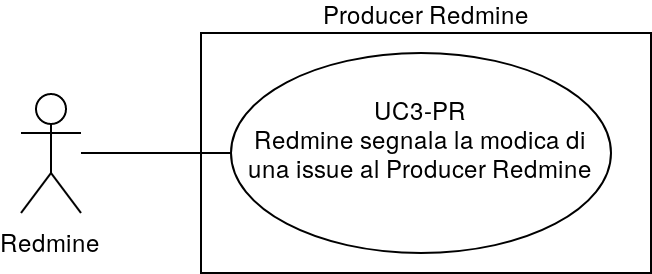
\includegraphics[width=0.5\textwidth]{img/casi_d'uso/UC3.png}\\
%		\caption{UC\theuccount-PR - Redmine segnala la modifica di una issue al Producer Redmine}
%	\end{figure}
	\begin{itemize}
		\item \textbf{Codice}: UC\theuccount-PR.
		\item \textbf{Titolo}: Redmine segnala la modifica di una issue al Producer Redmine.
		\item \textbf{Attori primari}: Redmine.
		\item \textbf{Descrizione}: quando una issue viene modificata, l'invio di tale segnalazione
		avviene da parte di Redmine tramite webhook.
		I campi di interesse sono gli stessi dell'apertura di una issue, con la differenza che necessariamente il campo status contiene ora ``updated''.
		\item \textbf{Precondizione}: Viene modificata una issue già aperta su un
		progetto di Redmine da segnalare a \progetto.
		\item \textbf{Postcondizione}: il Producer Redmine riceve la segnalazione da Redmine.
		\item \textbf{Scenario principale}: 
		\begin{enumerate}
			\item Viene modificata una issue già esistente su Redmine
			\item Redmine procede all'invio della segnalazione di modifica issue al Producer Redmine
		\end{enumerate}
		
	\end{itemize}